% Auto-generated LaTeX report for P5: Coherence Simulation
\documentclass[11pt,a4paper]{article}
\usepackage[utf8]{inputenc}
\usepackage{graphicx}
\usepackage{booktabs}
\usepackage{longtable}
\usepackage{hyperref}
\usepackage{geometry}
\geometry{margin=1in}
\title{Project 5 --- Coherence Protocol Evaluation}
\author{15346 Project Report}
\date{\today}

\begin{document}
\maketitle

\begin{abstract}
We evaluate five cache coherence protocols (MI, MSI, MESI, MOESI, MESIF) on a set of taskgraph traces. The experiments measure total simulator ticks across multiple processor counts to compare performance and scalability. This report summarizes the methodology, results, and insights about how additional coherence states affect performance for different sharing patterns.
\end{abstract}

\section{Introduction}
The goal of Project 5 is to introduce and evaluate multiple coherence protocols in the provided simulator. The handout requested testing at least four taskgraph traces, comparing performance across protocols and analyzing the benefit of additional coherence states (Shared, Exclusive, Owned, Forward).

\section{Methodology}
\subsection{Protocols}
We test the following coherence schemes (IDs used in the simulator):
\begin{itemize}
  \item MI (0)
  \item MSI (1)
  \item MESI (2)
  \item MOESI (3)
  \item MESIF (4)
\end{itemize}

\subsection{Workloads}
We used the provided taskgraph traces (12 traces in total). For the results presented in this report we focus on at least four representative traces: \texttt{blackscholes\\_4}, \texttt{dedup\\_4}, \texttt{dedup\\_8}, and \texttt{x264\\_8}.

\subsection{Configuration}
Each experiment used a simple cache configuration (4-way, block size 64B, sets=256) and varied the number of processors (2, 4, 8) and the coherence protocol. The simulator outputs total "Ticks" per run which we use as the primary performance metric (lower is better).

\section{Results}
\subsection{Overall Protocol Comparison}
Figure~\ref{fig:protocol} shows average ticks per protocol computed across all tested traces and processor counts. Table~\ref{tab:protocol_means} lists the protocol mean ticks (lower is better).

\begin{figure}[h!]
  \centering
  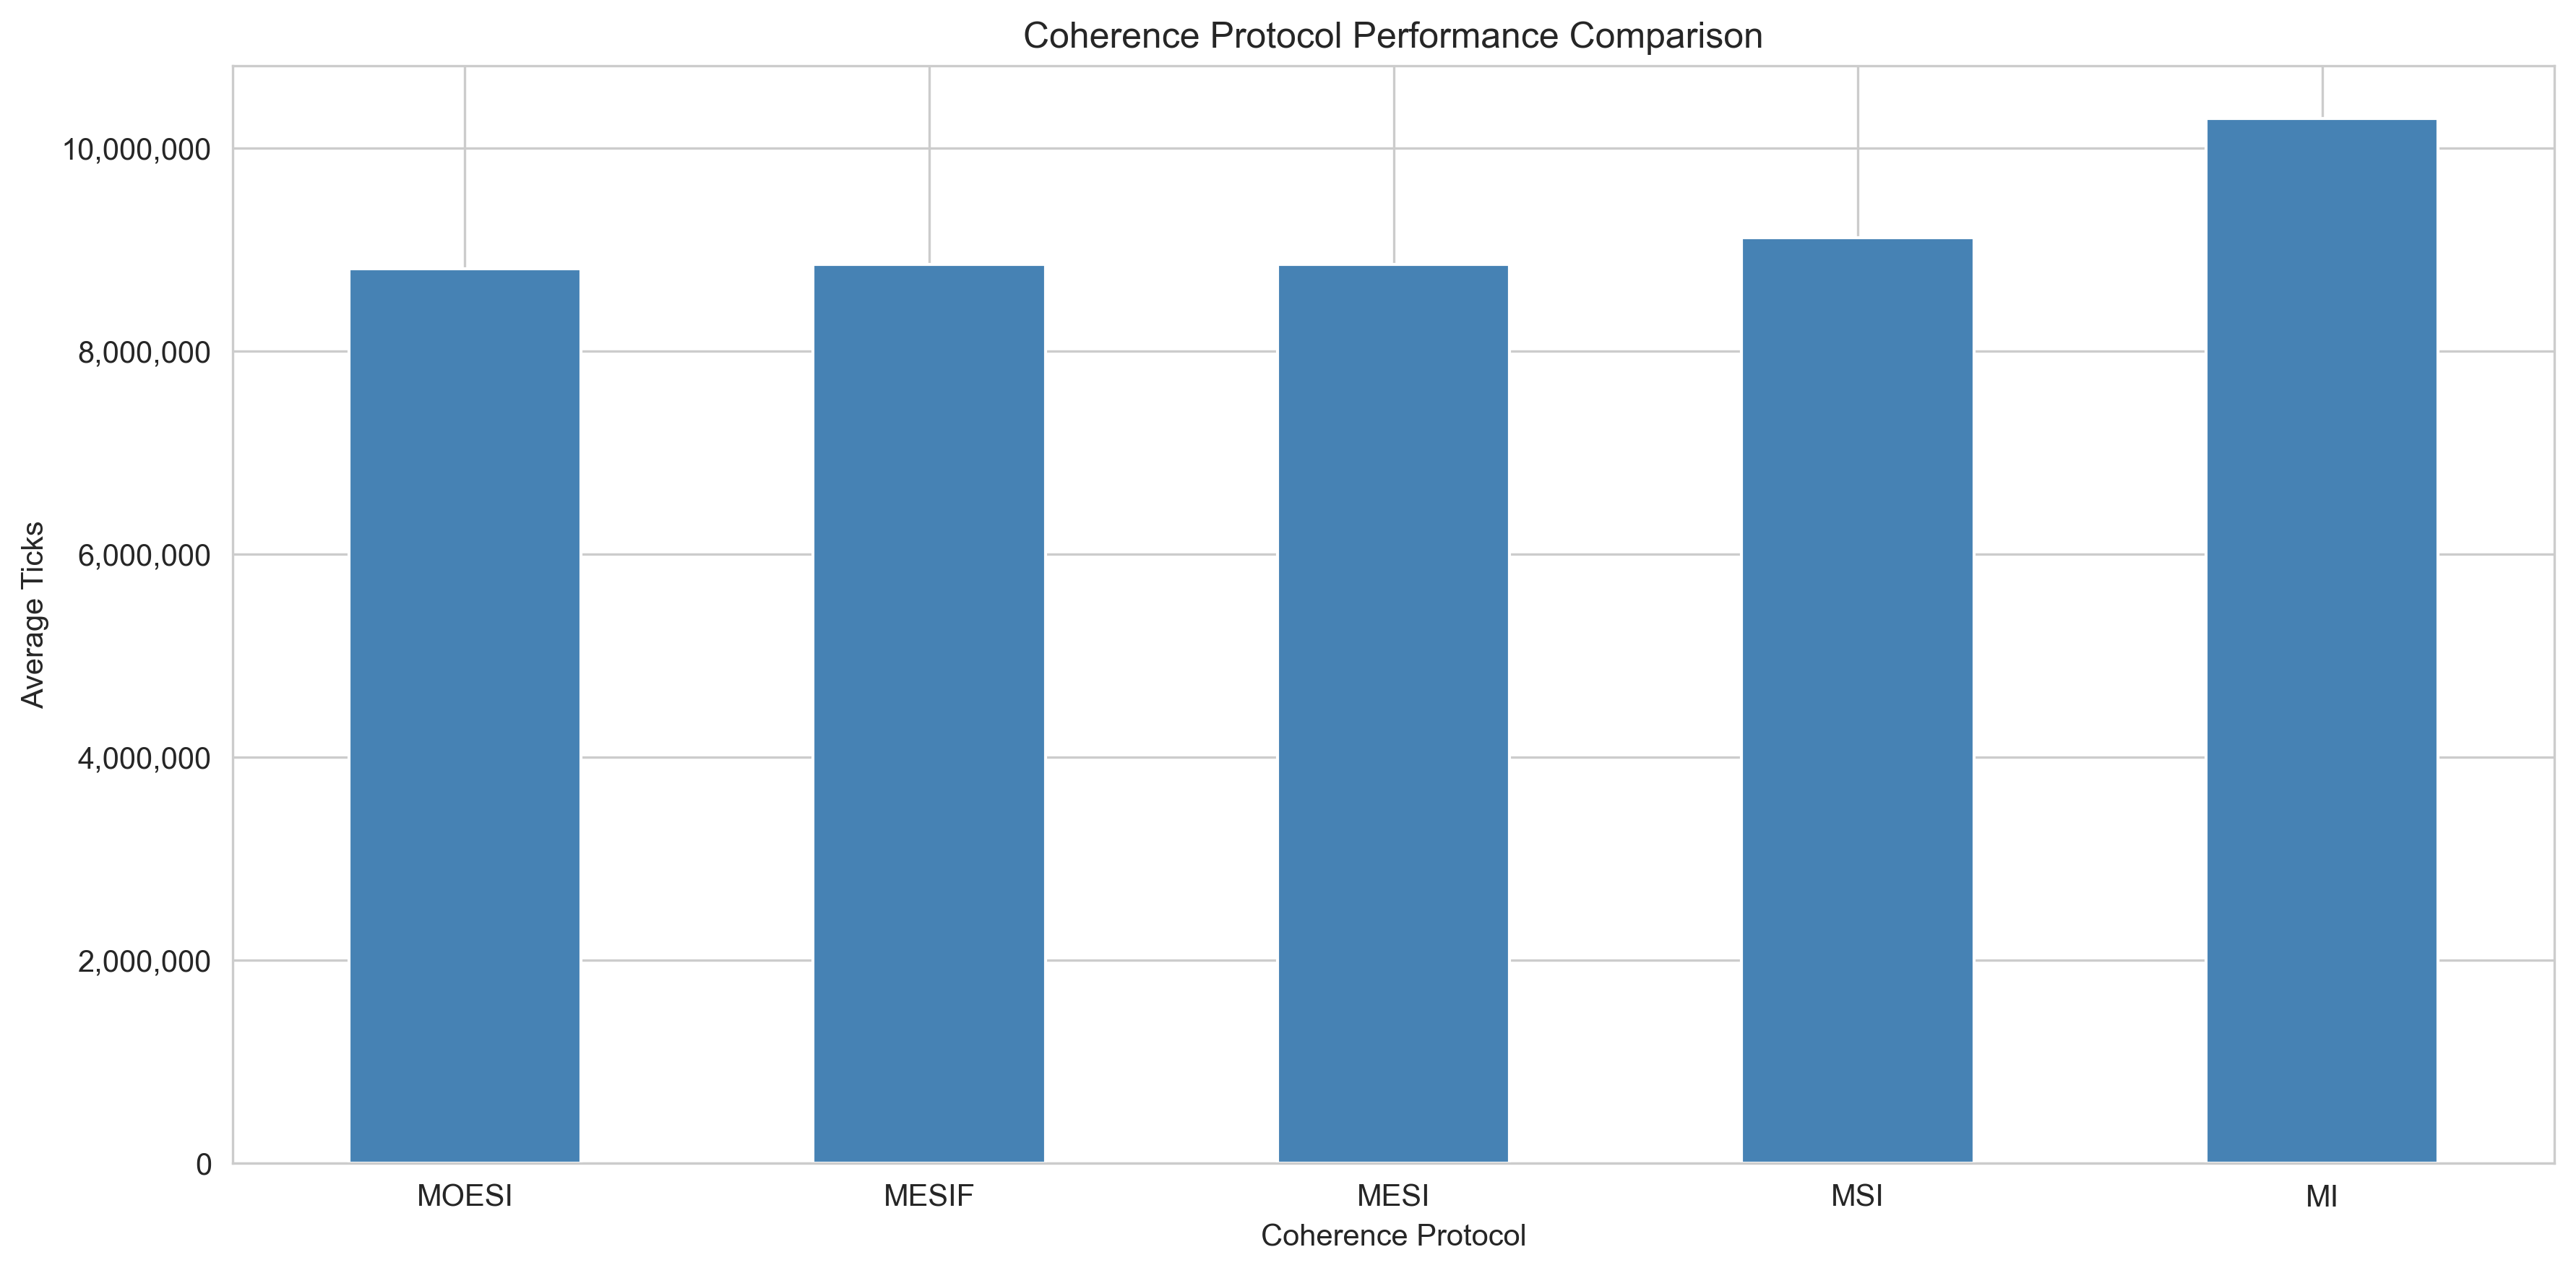
\includegraphics[width=0.75\textwidth]{experiment_results/figures/protocol_comparison.png}
  \caption{Average ticks by coherence protocol}
  \label{fig:protocol}
\end{figure}

\begin{table}[h!]
\centering
\caption{Mean ticks by protocol (averaged across traces and processor counts)}\label{tab:protocol_means}
\begin{tabular}{lrr}
\toprule
Protocol & Mean ticks & Improvement vs MI \\
\midrule
MOESI & 8,812,552.88 & 14.40\% \\
MESIF & 8,854,372.12 & 14.00\% \\
MESI  & 8,854,649.25 & 14.00\% \\
MSI   & 9,115,946.88 & 11.46\% \\
MI    & 10,295,600.38 & 0.00\% \\
\bottomrule
\end{tabular}
\end{table}

Discussion: MOESI provides the best average performance (about 14\\% improvement over MI). MESI and MESIF show near-identical improvements (~14\%), while MSI improves ~11.5\% over MI.

\subsection{Per-workload Analysis}
Table~\ref{tab:best_trace} reports which protocol performed best per representative trace, and the relative range across protocols.

\begin{table}[h!]
\centering
\caption{Best protocol per selected trace}
\label{tab:best_trace}
\begin{tabular}{lrrr}
\toprule
Trace & Best protocol & Best ticks & Worst ticks (range \\%) \\
\midrule
blackscholes\_4 & MESIF & 1,658,926 & 7,697,380 (78.45\%) \\
dedup\_4 & MI & 13,001,853 & 13,040,254 (0.29\%) \\
dedup\_8 & MI & 6,988,966 & 7,023,560 (0.49\%) \\
x264\_8 & MI & 13,494,202 & 14,648,837 (7.88\%) \\
\bottomrule
\end{tabular}
\end{table}

Discussion: Some workloads (e.g., \texttt{dedup\_4}, \texttt{dedup\_8}) show nearly identical performance across protocols, suggesting little benefit from extra coherence states. In contrast, \texttt{blackscholes\_4} achieves large gains (MESIF best) consistent with heavy read-sharing patterns where forwarding or exclusive states help.

\subsection{Scaling with Processor Count}
Figure~\ref{fig:scaling} visualizes protocol scaling with processor count. The table below summarizes mean ticks at 2 and 4 processors.

\begin{figure}[h!]
  \centering
  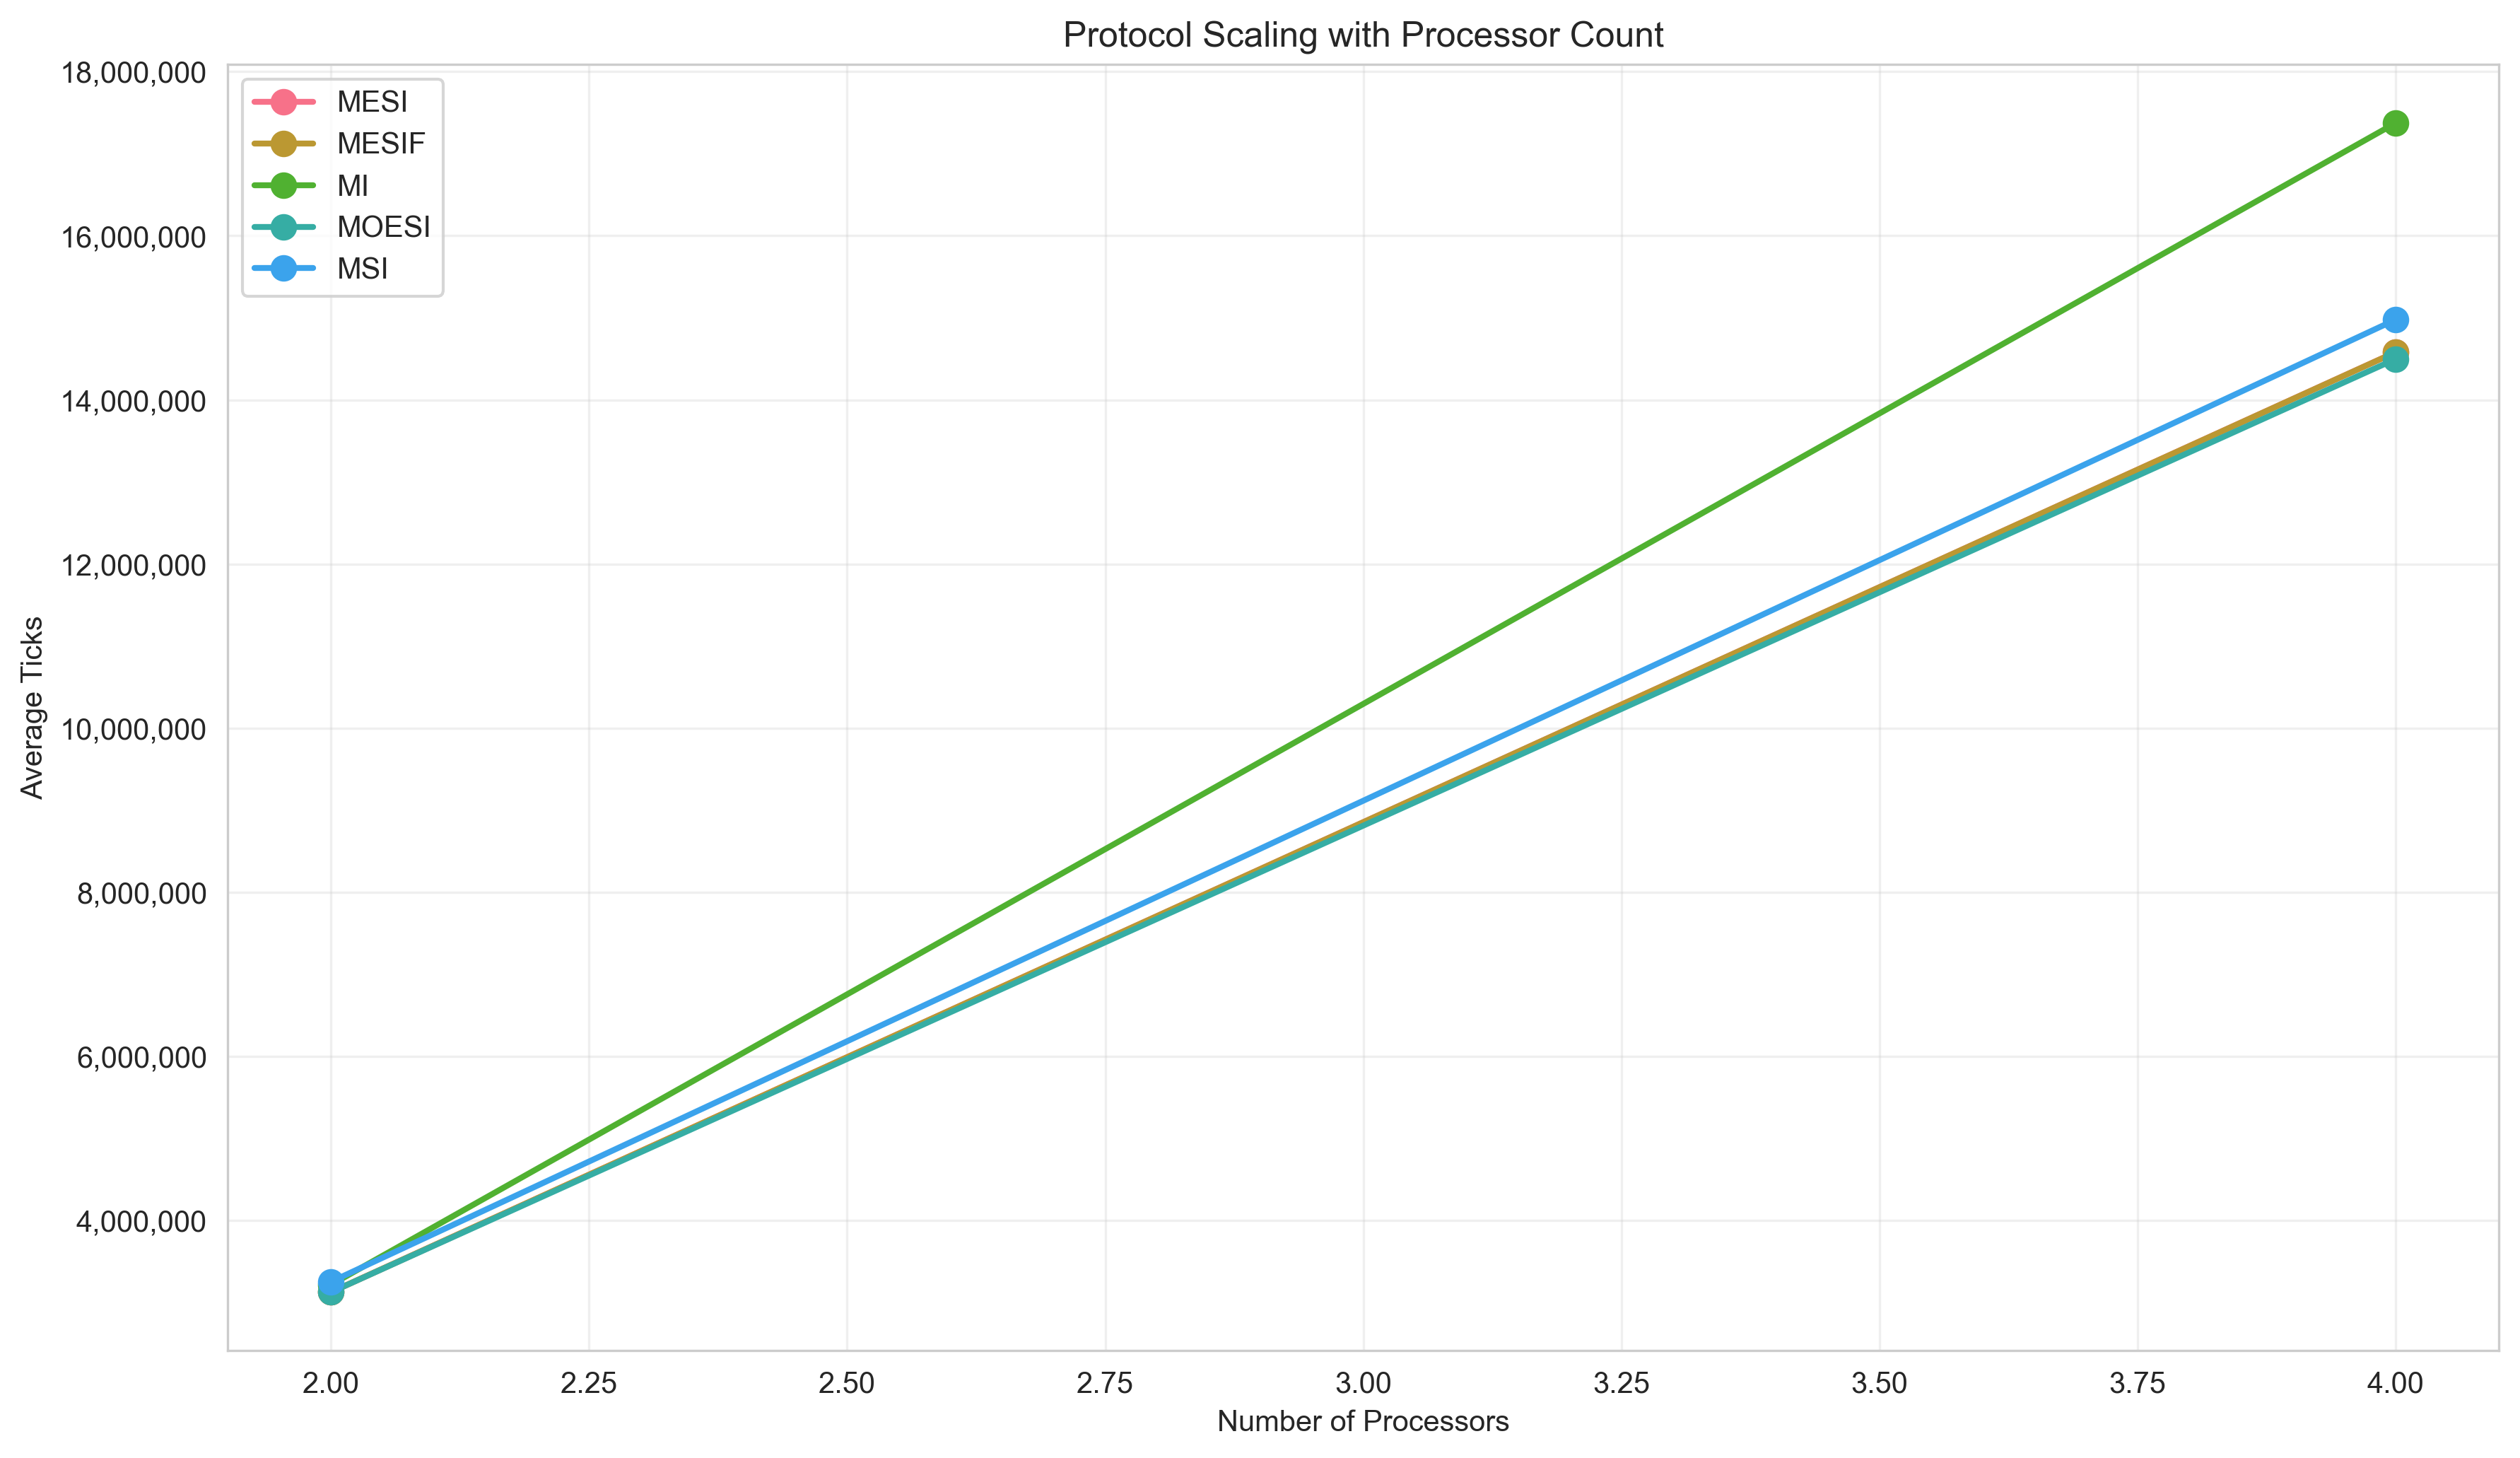
\includegraphics[width=0.75\textwidth]{experiment_results/figures/scaling_analysis.png}
  \caption{Protocol scaling vs. number of processors}
  \label{fig:scaling}
\end{figure}

\begin{table}[h!]
\centering
\caption{Mean ticks by protocol and processor count}
\begin{tabular}{lrr}
\toprule
Protocol & 2 processors & 4 processors \\
\midrule
MESI  & 3,127,734.50 & 14,581,564.00 \\
MESIF & 3,127,734.50 & 14,581,009.75 \\
MI    & 3,217,415.25 & 17,373,785.50 \\
MOESI & 3,127,498.50 & 14,497,607.25 \\
MSI   & 3,254,345.50 & 14,977,548.25 \\
\bottomrule
\end{tabular}
\end{table}

Discussion: All protocols show a substantial increase in ticks when moving from 2 to 4 processors for some traces; this reflects increased contention and synchronization overhead as more cores interact. MOESI/MESI/MESIF consistently give lower ticks at 4 processors than MI.

\subsection{Workload Heatmap and State Benefits}
Figure~\ref{fig:heatmap} shows the workload-protocol heatmaps (absolute and normalized) from the analysis.

\begin{figure}[h!]
  \centering
  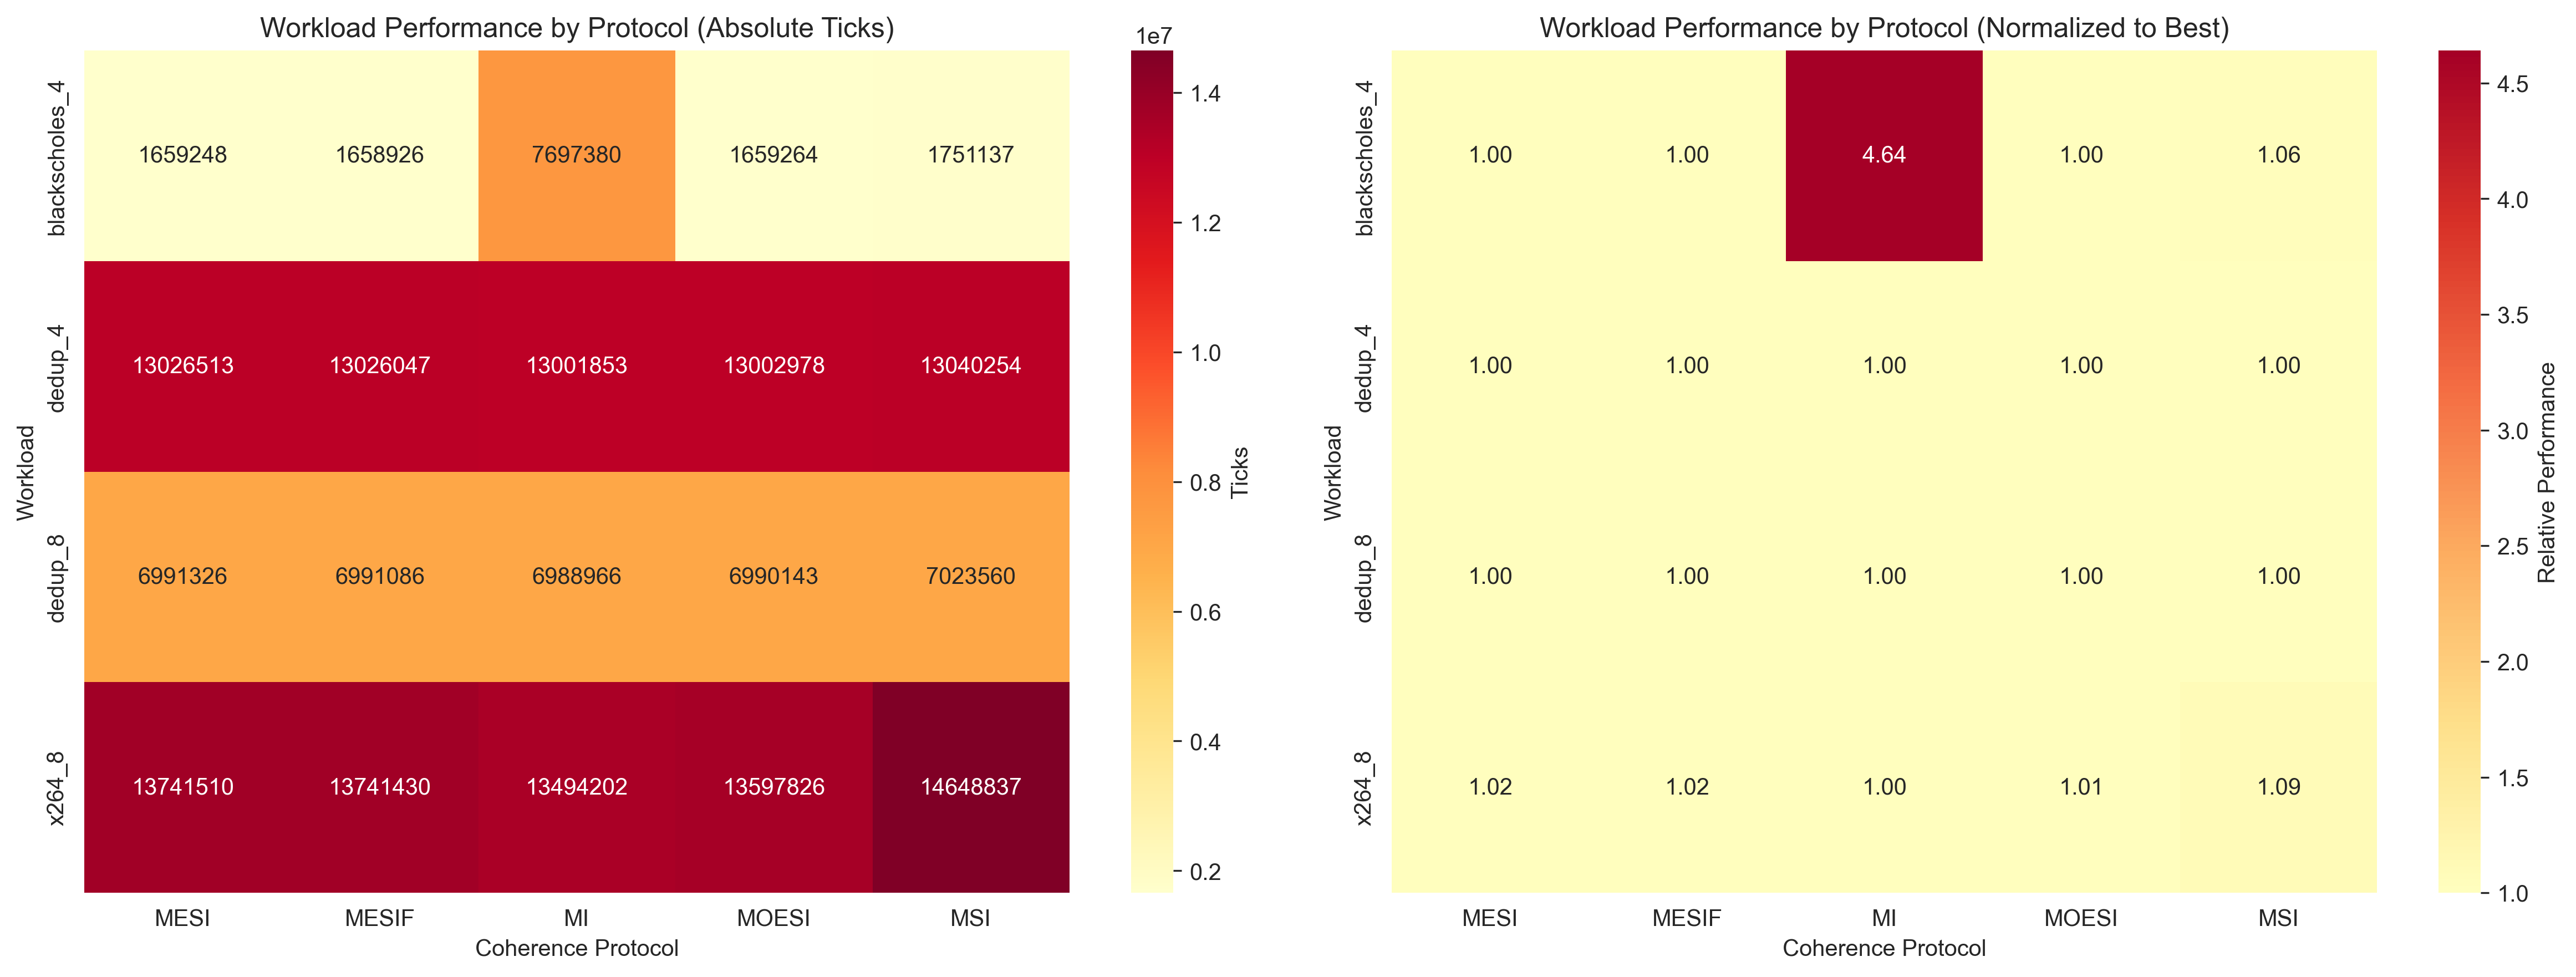
\includegraphics[width=0.9\textwidth]{experiment_results/figures/workload_heatmap.png}
  \caption{Workload performance heatmaps (absolute and normalized)}
  \label{fig:heatmap}
\end{figure}

Figure~\ref{fig:state_benefits} visualizes incremental benefits from adding states (S, E, O, F). The bar labels show percent improvement over MI.

\begin{figure}[h!]
  \centering
  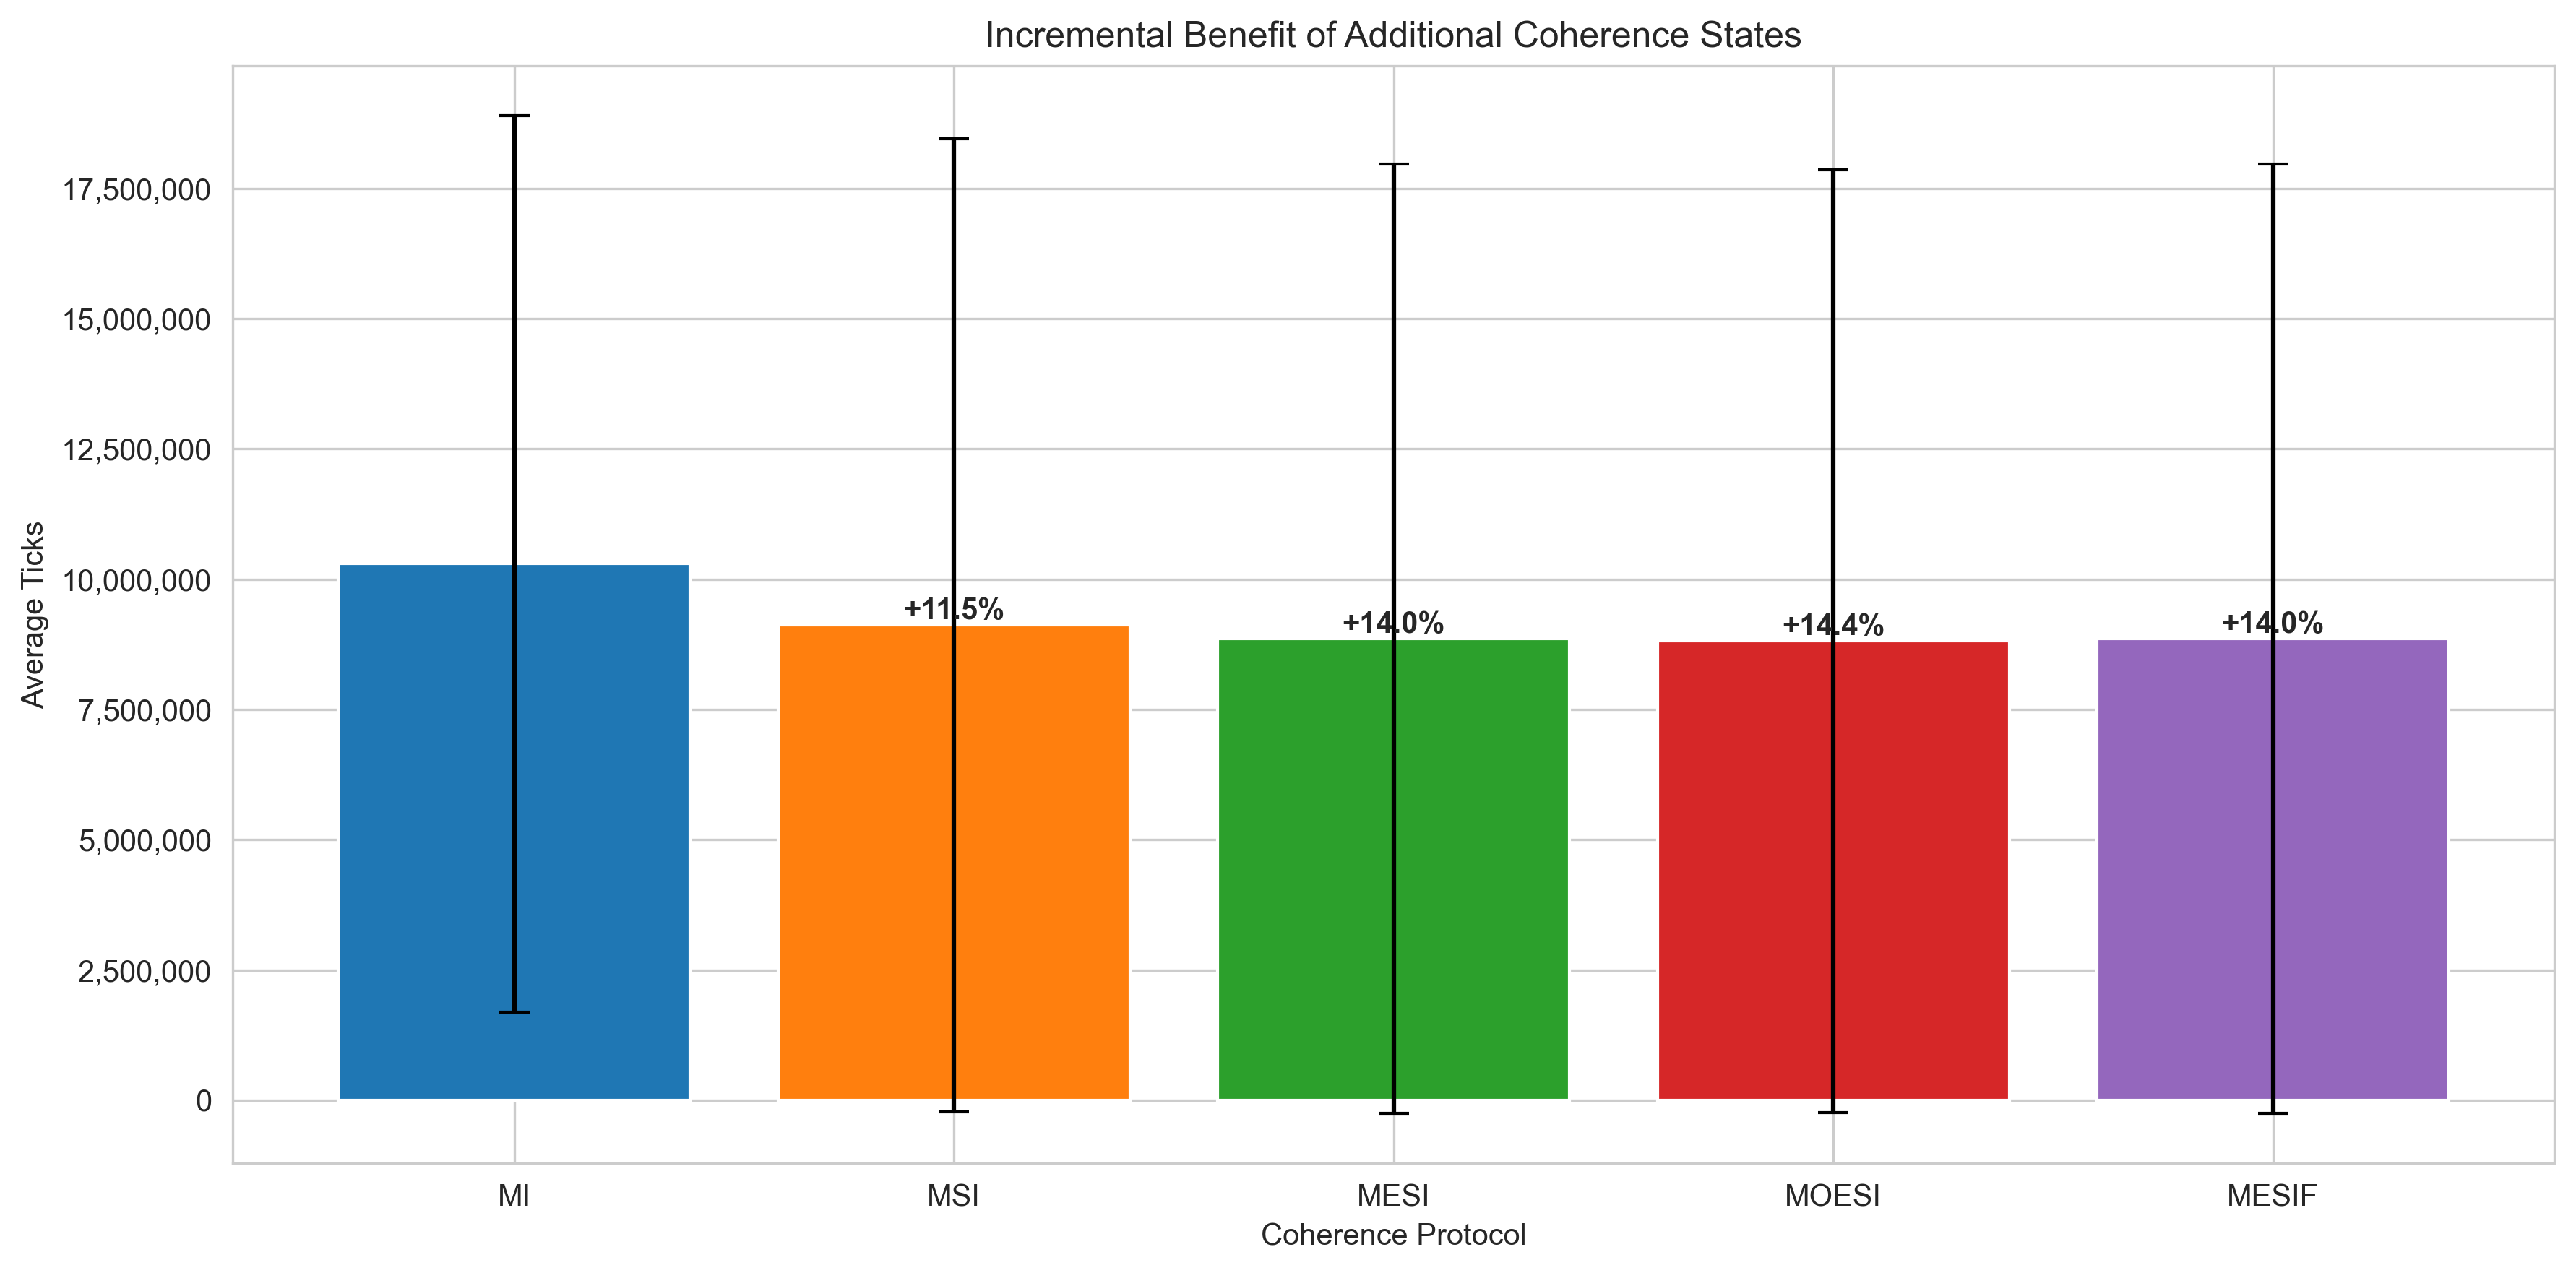
\includegraphics[width=0.75\textwidth]{experiment_results/figures/state_benefits.png}
  \caption{Incremental benefit of additional coherence states (average ticks)}
  \label{fig:state_benefits}
\end{figure}

\section{Conclusions}
Key findings:
\begin{itemize}
  \item MOESI provides the best average performance across traces in our experiments (~14\% improvement over MI).
  \item MESI and MESIF perform similarly on average; MESIF can be best on read-shared workloads (e.g., \texttt{blackscholes\_4}).
  \item Some workloads (e.g., the dedup traces) show negligible sensitivity to protocol choice, indicating limited sharing or balanced behavior where extra states provide little benefit.
  \item Protocol choice matters more as core count increases; MOESI/MESI/MESIF tend to scale better than MI.
\end{itemize}

\section{Appendix: Numeric Summary}
Below is the raw numeric summary generated from the experiment CSV (protocol means, best per trace, scaling):

\begin{verbatim}
Protocol summary (mean ticks):
                          mean           std      min       max  count
coherence_scheme                                                      
MOESI             8.812553e+06  9.044063e+06  1543775  24204885      8
MESIF             8.854372e+06  9.105729e+06  1543775  24250943      8
MESI              8.854649e+06  9.105935e+06  1543775  24251875      8
MSI               9.115947e+06  9.338068e+06  1613331  24277732      8
MI                1.029560e+07  8.599129e+06  1800871  24202835      8

Best protocol per trace:
               best_protocol  best_ticks  worst_ticks  range_pct
trace                                                           
blackscholes_4         MESIF   1658926.0    7697380.5  78.448175
dedup_4                   MI  13001853.0   13040254.0   0.294480
dedup_8                   MI   6988965.5    7023559.5   0.492542
x264_8                    MI  13494202.5   14648837.0   7.882090

Scaling (mean ticks by processor count):
processor_count            2            4
coherence_scheme                         
MESI              3127734.50  14581564.00
MESIF             3127734.50  14581009.75
MI                3217415.25  17373785.50
MOESI             3127498.50  14497607.25
MSI               3254345.50  14977548.25
\end{verbatim}

\end{document}
